
%(BEGIN_QUESTION)
% Copyright 2010, Tony R. Kuphaldt, released under the Creative Commons Attribution License (v 1.0)
% This means you may do almost anything with this work of mine, so long as you give me proper credit

Calculate the required fluid velocity in order to reduce the pressure at the narrow throat to 0 PSIG, then also calculate the volumetric flow rate corresponding to this velocity in units of GPM:

$$\includegraphics[width=15.5cm]{i00052x01.eps}$$

The inside diameter (ID) of the throat is 1 inch, while the inside diameter of the wide pipe is 4 inches.  Assume the fluid to be water ($\rho$ = 1.94 slugs/ft$^{3}$) at a constant downstream pressure of 10 PSIG:

\vfil

Hint: the trick to solving for velocity ($v$) is to reduce Bernoulli's equation so that it contains just that one unknown variable.  In other words, you need to be able to express the velocity at the 1-inch throat in terms of the velocity at the 4-inch pipe, so you will have just one $v$ in the equation rather than a $v_1$ and a $v_2$.

\underbar{file i00052}
\eject
%(END_QUESTION)





%(BEGIN_ANSWER)

This is a graded question -- no answers or hints given!

%(END_ANSWER)





%(BEGIN_NOTES)

$P_1$ = 1440 pounds per square foot

\vskip 10pt

The ``trick'' to solving for $v$ is to reduce the number of unknown variables in the equation.  At first we have two unknown velocities, $v_1$ and $v_2$, which is too many to solve for.  However, since we do know the pipe diameters at both locations, we may express the velocity at the 1-inch throat in terms of $v$ at the 4-inch pipe, thereby eliminating one of the unknown $v$ quantities.  Since the diameter ratio is 1:4, and area ratio will be 1:16, which means the velocity ratio must be 16:1.  Thus, the velocity at the 1-inch throat is $16v$ if the velocity at the 4-inch pipe is $v$:

$$z_1 \rho g + {1 \over 2} \rho v_1^2 + P_1 = z_2 \rho g + {1 \over 2} \rho v_2^2 + P_2$$

$${1 \over 2} \rho v^2 + 1440 = {1 \over 2} \rho (16v)^2$$

$$1440 = {1 \over 2} \rho \left[ (16v)^2 - v^2 \right]$$

$$1440 = {1 \over 2} \rho \left[ 256v^2 - v^2 \right]$$

$$1440 = {1 \over 2} \rho (255v^2)$$

$${2880 \over {255 \rho}} = v^2$$

$$v = \sqrt{{2880 \over {255 \rho}}}$$

$$v = \sqrt{{2880 \over {255 \times 1.94}}} = 2.4128 \hbox{ ft/s}$$

\vskip 10pt

Once we know the velocity at the throat, we may calculate the volumetric flow rate using the $Q = Av$ continuity equation (and then converting from units of cubic feet per second into gallons per minute):

\vskip 10pt

$Q$ = 94.5052 gallons per minute

%INDEX% Physics, dynamic fluids: Bernoulli's equation

%(END_NOTES)


